% !TeX spellcheck = en_US
\documentclass{article}
\usepackage{authblk}
\usepackage{float}
\usepackage{amsmath}
\usepackage{amssymb}\usepackage{amsthm}
\usepackage{mathtools}
\usepackage{xspace}
\usepackage{xcolor}
\usepackage{graphics}
\usepackage{tabu}
\usepackage{accents}
\usepackage{algorithmicx}
\usepackage{algpseudocode}
\usepackage[plain]{algorithm}
\usepackage{tikz}
\usetikzlibrary{shapes, arrows}
\usetikzlibrary{arrows.meta,bending,positioning,decorations.text}
\usepackage[
backend=biber,
style=numeric,
doi=true,
isbn=false,
url=false,
eprint=false,
sorting=ynt
]{biblatex}
\addbibresource{Community.bib}
\addbibresource{Disease_module.bib}
\addbibresource{Network_Medicine.bib}
\addbibresource{Genomic_Database.bib}
\addbibresource{Software.bib}

%% COMMENTARIES DEFINITION ========================================
\newif\ifcomment
\commenttrue
% \commentfalse
\newcommand{\mycomment}[2]{
\ifcomment
{\noindent \small \textbf{#1:} \color{black!90!white} {#2}}}
\newcommand{\FD}[1]{\mycomment{\color{red!50!black}{Franck}}{#1}}
\newcommand{\CB}[1]{\mycomment{\color{orange!80!black}{Celia}}{#1}}

\newtheorem{theorem}{Theorem}
\newtheorem{proposition}{Proposition}
 
\newcommand{\tuple}[1]{\langle #1 \rangle}
\newcommand{\Bool}[0]{\mathbb{B}}
\newcommand{\Nat}[0]{\mathbb{N}}
\newcommand{\Real}[0]{\mathbb{R}}
\newcommand{\doot}[1]{\accentset{\bullet}{#1}}

\newcommand{\ie}[0]{\textit{i.\,e., }\xspace}
\newcommand{\eg}[0]{\textit{e.\,g., }\xspace}

\newcommand{\email}[1]{\texttt{#1}\relax}

\DeclareMathOperator*{\argmax}{\arg\,\max}
\DeclareMathOperator*{\argmin}{\arg\,\min}

\definecolor{color1}{rgb}{0.55, 0.83, 0.54}
\definecolor{color2}{rgb}{0.89, 0.42, 0.38}
\definecolor{color3}{rgb}{1, 0.86, 0.13}

\DeclareMathOperator{\counts}{\mathbf{Count}}

\newcommand{\chrocode}[0]{\textsc{chrocode}\xspace}

%% 
\newcommand{\entryneedsurl}[1]{\addtocategory{needsurl}{#1}}

\begin{document}

\title{Chromatic Community Structure Detection}


\author{Franck Delaplace}
\affil{\textsc{ibisc}-lab, Paris-Saclay University, Univ. Evry 
\email{franck.delaplace@univ-evy.fr}
}


	
\date{}

\maketitle{}
%\begin{center}
%\textcolor{red}{\textsc{\huge - confidential -} }
%
%\textcolor{red}{\large \sc do not distribute}
%
%\end{center}
 
\begin{abstract}
{The detection of community structure is probably one of the hottest trends in complex network research as it reveals the internal organization of people, molecules or processes behind social, biological or computer networks\dots The issue is to provide a network partition representative of this organization so that each community presumably gathers nodes sharing a common mission, purpose or property.
Usually the identification is based on the difference between the connectivity density of the interior and the boundary of a community. Indeed, nodes sharing a common purpose or property are expected to interact closely. Although this rule appears mostly relevant, some fundamental scientific problems like disease module detection highlight the inability to determine significantly the communities under this connectivity rule. The main reason is that the connectivity density is not correlated to a shared property or purpose. Therefore, another paradigm is required for properly formalize this issue in order to meaningfully detect these communities. In this article we study the community formation from this new principle. Considering colors formally figures the shared properties, the issue is thus to maximize group of nodes with the same color within communities.. We study this novel community framework by introducing new measurement called \emph{chromarity} assessing the quality of the community structure regarding this constraint. Next we propose an algorithm solving the community structure detection based on this new community formation paradigm.}

\medskip
\noindent
\textbf{Keywords: }{Community structure, Detection algorithm.}
\end{abstract}

\section{Introduction}

%% CONTEXT
Complex networks model component interactions in diverse real-world domains as in sociology with social or friendships networks, computer science with WEB, and biology with regulatory, metabolic or neural networks. Nodes of these networks are often arranged in closely tight groups called communities.
These communities delineate the organizational supports of function, property, purpose or categories. They thus highlight a structure of the network providing an organizational understanding behind the topology. 
 Formally, the goal is to identify a node partition of the nodes of the network. A \emph{community structure} is a partition of the vertices of a graph defined according rules structuring the vertex distribution. Although there is no firm answer concerning these rules~\cite{fortunato2016}, it is commonly admitted that the definition of a community relates to a difference in connection density between its interior and its boundary. The density of connection between nodes inside a community must be higher than the density of connection across communities. Such community obtained by this method is called the \emph{topological community}~\cite{liu2014}. 
Community detection algorithms capture this difference of connection density for detecting communities in a network~\cite{fortunato2010, khan2017}. The quality of a community structure is evaluated by a measure assessing this partitioning rule. A recognized standard is the \emph{modularity} introduced by Newmman~\cite{newman2006}. The modularity is based on the comparison of the network with a random one having the same topological characteristics than the original one (\ie same number of nodes, same node degree). Therefore a good measure must be greater than a community structure having the same characteristics but obtained by chance because this reveals an organizational bias. Finding a community structure maximizing the modularity is NP-hard~\cite{brandes2006} and different heuristics have been proposed for detecting the best community structure~\cite{pons2005,blondel2008,fortunato2010,murata2010}.

%% Expliquer la limite: Disease module 
While the concept of community is central in network science, the connection density rule fails to significantly identify the meaningful community structure of a network for some issues, thus restricting the applicability of community detection algorithms. It is notably the case for \emph{disease module} discovery. 
 A disease module groups genes which are mechanistically linked to the same patho-phenotype.The study of the modularity of human disease would provide a causal understanding of the pathogenesis strengthening the etiological explanation and rationally determine clues for drug target discovery. 

In \cite{ghiassian2015}, the authors carefully demonstrate that disease module are not topological module/community. By using three representative, methodologically distinct algorithms on community structure detection based on density connection, the authors show that the disease genes gathered in a community by connection density method are drastically under-represented, thus prohibiting the ability to assign communities to diseases. Moreover, they also show that this lack of representativeness is not due to an insufficiency of knowledge about genetic diseases, but rather to the inadequacy of the density connection method to properly address the disease module. This empirical analysis is explained by the authors by the fact that the disease proteins do not form particularly dense subgraphs. This conclusion is also confirmed by other works on the disease module domain~\cite{sharma2015,silberberg2017,pavan2017} which propose alternative clustering methods based on other rules than those governing topological community detection. 

Because of its overarching importance in health, the identification of disease modules clearly states the need to extend this framework for detecting community structures by including other categories of problems. Therefore, based on the disease module, our objective is to generalize its principles from the proposed method in order to characterize an alternative community detection paradigm. 

\textsc{diamond}~\cite{ghiassian2015}, \textsc{gladiator}~\cite{silberberg2017}, and \textsc{sca}~\cite{wang2018} are three computational methods solving the disease module detection based on different approaches. However, they share some common features allowing us to state the fundamental rules for finding disease module. 

The genes implicated in a disease are retrieved from databases analysis as \textsc{omim}\cite{hamosh2005,amberger2015a} for Mendelian diseases or \textsc{orphanet}~\cite{pavan2017} for orphan diseases. They constitute the landmarks of the disease at molecular level and reciprocally a fundamental property assigned to these genes from which the disease module can be detected. Hence this property is central and monitor the community structure detection. 

A backbone of network biology lies on the ``local hypothesis'' stating that genes or proteins involved in the same disease have a tendency to interact with each other~\cite{furlong2013b} and to cluster in the same neighborhood \cite{oti2006,barabasi2011}. Hence, all disease related genes in a module are necessary connected together over a short distance. Connectivity analysis depends on algorithmic methods, and two disease-related genes may or may not be considered neighbors. \textsc{diamond} examines the neighborhood of gene by identifying a typical connection pattern that must differ to random/null model connection. They are thus looking for a characteristic connectivity pattern between disease genes. The connection rules of \textsc{gladiator} are based on the reproduction of connection obtained by phenotypic similarity analysis, while \textsc{sca} reconnects the disease seeds by few extra hidden nodes qualified as seed connectors while complying with a short connectivity distance between seeds. 

All these algorithms aims at finding the largest modules encompassing the greatest number of genes related to a disease, and stop when no improvements are possible. Therefore the definition of a module relates here to largest number of connected nodes which mostly share the same property. 

Disease module detection exemplifies an important problem for community structure inference where the condition underpinning the node partition is related to alternative criteria than connection density difference between the interior and the boundary of a community. Therefore, it seems greatly beneficial for extending the scientific questioning on network community that the resolution of this problem is achieved in a broader context than disease modules, impelling to generalize the statement of this problem.

The common property which is responsible for the formation of the community must be understood in a broad sense including a wide variety of situations such as involvement in the same process or function, membership of a social or ethnic group, identical characteristics, sharing a common topic of interest, common purpose or mission etc., more generally any trait that can be shared by a community and qualifying its members. This property will be formally assimilated to a ``color'' leading to assigning the same color to the nodes having the same property. Accordingly, the issue of \emph{chromatic community structure} detection is to find communities of connected nodes that maximize the density of the major color within each. 

Such problem statement explains why the connection density based algorithms may fail to detect such communities because the nodes with the same colors can be sparsely connected since only the connectedness prevails and potentially separated by nodes differently colored. As there is no a priori relationships between colors and connections, nodes with the same color can be located through communities obtained by connection density rule. 

In this article, we study the chromatic community structure detection problem and propose an algorithm for finding partition of communities. In Section~\ref{sec:formalization} we mathematically formalize the problem. We then define in Section~\ref{sec:chromarity} the \emph{chromarity} which is a measure assessing the quality of a chromatic community structure. We detail in Section~\ref{sec:chrocode} an algorithm finding a chromatic community structure. The algorithm is then evaluated in Section~\ref{sec:benchmark} before concluding (Section~\ref{sec:conclusion}). 


\section{Formalizing the coloring}
\label{sec:formalization}
In this section we address the basic notions related graph coloring. 
Let $G=\tuple{V,E}$ be a graph where $V$ is a set of vertices and $E \subseteq V \times V$ a set of edges, a \emph{community} $p$ is a subset of $V$ (\ie $p \subseteq V$) and a \emph{community structure} $P$ is a partition of $V$, namely:
\begin{equation*}
\bigcup_{p_i \in P} p_i = V \land \forall p_i,p_j \in P: p_i \cap p_j \neq \emptyset \implies p_i = p_j.
\end{equation*}
A community structure based on color selection criteria is called a \emph{chromatic community structure}. 

\paragraph{Coloring profile.} Coloring assigns a color to each vertex of a graph which is described by a \emph{coloring profile} corresponding to an application from vertex to color $c: V\to C$ where $C$ denotes the set of colors. The set of colors $C$ will be represented by an integral interval $[1,r]$ where integers define colors. For example $c=\{1 \mapsto 1 , 2 \mapsto 1, 3 \mapsto 2, 4 \mapsto 3 , 5 \mapsto 3 \}$ assigns color $1$ to nodes $1,2$, color $2$ to node $3$ and color $3$ to nodes $4,5$.
The restriction of the coloring to community denoted $c_p$ for community $p \subseteq V$ is defined as: 
$c_p=\{ v \mapsto c(v) \mid v \in p \}.$
 
If the vertices correspond to an integral interval $V=[1,n]$ then the coloring profile can be described by a vector such that the index stands for a vertex label and its corresponding value for a color (\ie $c(i)=k \iff i \mapsto k \in c$). For example $c=\{1 \mapsto 1 , 2 \mapsto 1, 3 \mapsto 2, 4 \mapsto 3 , 5 \mapsto 3 \}$ is described by the vector $(1,1,2,3,3)$.

\paragraph{Colored Graph.} A \emph{colored graph} is a $3-$uple $\tuple{V,E,c}$. The colored graph in Figure~\ref{fig:community structure} uses $3$ colors $C=[1,3]$ where: green$=1$, red$=2$ and yellow$=3$. From its coloring profile: 
$$c=\{1 \mapsto 1, 2 \mapsto 3, 3 \mapsto 1, 4 \mapsto 2 , 5 \mapsto 1, 6 \mapsto 3 \}$$ 
the vector representation is $(1,3,1,2,1,3)$. Given the following chromatic community structure:
$$P= \{ p_1=\{ 1,3,4,5\}, p_2=\{2,6\} \},$$, 
we deduce the following coloring profiles restricted to $p_1, p_2$: 
$$c_{p_1}= \{ 1 \mapsto 1, 2 \mapsto 3, 4 \mapsto 2, 5 \mapsto 1\}, c_{p_2}= \{2 \mapsto 3, 6 \mapsto 3\}.$$
\begin{figure}[htb]
	\centering
	\includegraphics[width=0.5\textwidth]{image/gintro.png}
	\caption{Community structure of a colored graph.}
	\label{fig:community structure}
\end{figure}

\paragraph{Transparency.}

 The absence of properties of a vertex is represented by the \emph{ transparency} (denoted $0$) since a color is assumed to qualify a property or an attribute of a vertex. The transparency is not a color \ie $0 \notin C$. Transparent vertices are thus never involved when it comes to color, but the transparent vertices still exist as vertices.

\paragraph{Chromatic function.} A \emph{chromatic function} $\chi: (V \to C) \to C \to \Nat$ counts the number of occurrences of each color in a coloring profile. The formal definition of the chromatic function is based on the \emph{counting operator} $(\counts)$ which is a function counting the positions/nodes of each element corresponding to values of a vector or a function. $\counts(X,y)$ specifically counts the number of occurrences of element $y$ in vector/function $X$:
\begin{equation*}
\begin{split}
\counts(X,y) &= \left\{ y \mapsto \big|\{ i \mid X(i) =y \} \big| \right\}.\\
\counts(X) &= \bigcup_{i=1}^{|X|} \counts(X,X(i)).
\end{split}
\end{equation*}
 The chromatic function is thus defined from a coloring profile $c$ as:
\begin{equation}
\chi_{c}= \bigcup_{k \in C} \counts(c,k)
\label{def:chromatic function}
\end{equation}
The chromatic function of $c$ of the example in Figure~\ref{fig:community structure} is: $$\chi_{c}=\{ 1 \mapsto 3, 2 \mapsto 1, 3 \mapsto 2 \}.$$
For the following coloring profile $c=(0,0,1,2,1,0,1,3,0,3)$ with transparent color, we also have the same chromatic function because the transparency is not accounted as color by definition~(\ref{def:chromatic function}) since $0 \notin C$.

Finally, the density also includes the transparency since it corresponds to the ratio of the number $d$ of vertices with the same color by the number $n$ of vertices in a community ($\frac{d}{n}$). As example, from the previous coloring profile with transparency, the density of color $1$ ($d=3$) is $\frac{3}{10}=0.3$.

\paragraph{Dominant color.} A coloring profile with $d$ vertices of the same color, will be called a \emph{ $d-$coloring profile}. This notion is also applied to community from their local coloring profile. A \emph{$d-$colorful community} $p$ implies that:
\begin{equation}
\exists k \in C: \chi_{c_p}(k)=d.
\label{def: d colored community}
\end{equation}
Notice that these coloring profiles may also have several subsets of vertices with the same color of cardinality greater or equal to $d$. The graph in Figure~\ref{fig:community structure} is a $3-$coloring profile for color $1$, but also a $2-$coloring profile for color $3$, and $1-$coloring profile for color $2$.

\medskip
Among the $d-$coloring profiles we specifically focus on the class of profiles where $d$ is the cardinality of the color occurring the most. These profiles are said \emph{$d-$dominant} by this main color. Hence a coloring profile is $d-$dominant if and only if:
\begin{equation}
\exists k \in C: \chi_{c}(k)= d \land \forall k' \in C: \chi_{c}(k') \leq d.
\label{def:d dominant community}
\end{equation}
In this case, color $k \in \argmax \chi_{c_p}$ is said \emph{dominant}. In Figure~\ref{fig:community structure} the dominant color is $1$ and the coloring profile is thus $3-$dominant. By extension, a community is said $d-$dominant if the restriction of the coloring profile to this community is $d-$dominant. In Figure~\ref{fig:community structure}, $p_1$ is $3-$dominant for color $1$ and $p_2$ is $2-$dominant for color $3$. 
%% As the color dominates in size we deduce that: $d \geq \left \lceil \frac{|p|}{|C|} \right \rceil$. 
Notice that several dominant colors may exist in a coloring profile. 


\section{Chromarity}
\label{sec:chromarity}
A meaningful chromatic community structure maximizes the occurrence of the dominant color within each community. 
The quality of a chromatic community structure is quantitatively assessed from a measure quantifying this maximization.
Accordingly, the density of the dominant color is worth considering as a basic measure because it assesses the size of a dominant color relatively to the size of the community, calculated as: $\frac{\max \chi_{c_p}}{|p|}$. By contrast to the mere count of the dominant color, the density allows comparison of communities of different sizes by primarily analyzing the occupancy rate of a color within them. Therefore it does not necessary privileged the larger communities but rather the communities with an high occupancy rate of a specific color.

However, adopting the density as the basic measurement for assessing the quality of a chromatic community structure leads to a trivial non informative optimal solution restricting all communities to a single node. Inside each community the color of the single node therefore covers the entire community leading to an optimal density of $1$ for all communities, thus with an optimal overall mean density of $1$. This community structure however clearly tells us nothing of value about community organization since all nodes are isolated,, and therefore no informative structure is inferred. 
The single-node community division scenario shows that merely maximizing the density of the dominant color is not a good way for quantifying the intuitive notion of chromatic community structure.

A good division of a graph not only improves the dominant color density; it is one having a higher density than one would expect by chance. Indeed, situation that cannot be delivered by chance underpins an intentional or mechanistic organization. As a result, we can safely conclude that the structure of the chromatic community excluding the chance provides a meaningful structure because it clearly demonstrates intentional design.

The \emph{chromarity} will quantify the measure of a community structure related to chance. Informally, the chromarity assesses the expectation of obtaining a random free density of dominant color.
To define it, we will first evaluate the probability of having a $d-$colored community of size $n$ of a particular color chosen among $|C|=r$ colors by chance. This probability is the ratio of the favorable cases to the possible cases.
The number of the whole possible colored communities is $r^n$ corresponding to the cardinal of the complete enumeration of the possible combinations of vertex coloring with color repetitions among $r$ colors. 
Concerning the favorable cases, two issues are addressed providing two different chromarities here: 
\begin{enumerate}
\item the enumeration of the $d$-colorful communities or color profiles of size $n$ with $r$ colors; \label{issue:1}
\item the enumeration of the $d-$dominant colorful communities or colors profiles of size $n$ with $r$ colors. \label{issue:2}
\end{enumerate}
The first issue does not impose the domination but just the cardinality of a subset of vertices with the same color while the second refers exactly to the definition of a $d-$dominant coloring profile.
The separation of the enumeration problem in two issues is motivated by the computational complexity of the resulting combinatorial formulas explained in Section~\ref{sec:benchmark}.
 We thus need to enumerate the favorable colorful communities for each issue. Subsection~\ref{sec:enumeration kappa} defines the combinatorial formula enumerating the favorable colorful communities for issue~\ref{issue:1}, while 
 Subsection~\ref{sec:enumeration gamma} determines it for issue~\ref{issue:2}. 
 
\subsection{Enumeration of $d-$colorful communities}
\label{sec:enumeration kappa}
Different coloring of $d$ vertices are obtained using any color. Let $D_k$ be the set of colorful communities having $d$ vertices of color $k$, the count of all communities containing a $d-$color profile obviously corresponds to the cardinality of the union of these sets, namely: $|\bigcup_{k=1}^r D_k|$. Some communities may have a $d$-color profile for different colors, meaning that these sets intersect. The enumeration formula of $|\bigcup_{k=1}^r D_k|$ is based on the \textit{Poincar\'e sieve} (inclusion-exclusion principle), for the cardinal of the union: 
$$\left|\bigcup_{k=1}^r D_k \right|= \sum_{k=1}^r (-1^k) \sum_{1\leq i_1 \leq \cdots \leq i_j \leq \cdots \leq i_k \leq r} | D_{i_1} \cap \cdots \cap D_{i_j} \cap \cdots \cap D_{i_k}|$$.

For example let us considering $3$ sets, from the \textit{Poincar\'e sieve} the cardinal is then~(see Figure~\ref{fig:venn diagram union 3 sets})
\begin{multline*}
|D_1 \cup D_2 \cup D_3| = |D_1|+ |D_2| + |D_3| \\- ( |D_1 \cap D_2| + |D_1 \cap D_3| + |D_2 \cap D_3|) \\+ |D_1 \cap D_2 \cap D_3|.
\end{multline*}

To obtain the formula enumerating the $d-$colorful communities, we thus need to define a combinatoric formula for each set and each intersection of sets. 

\begin{figure}[htb]
	\centering
	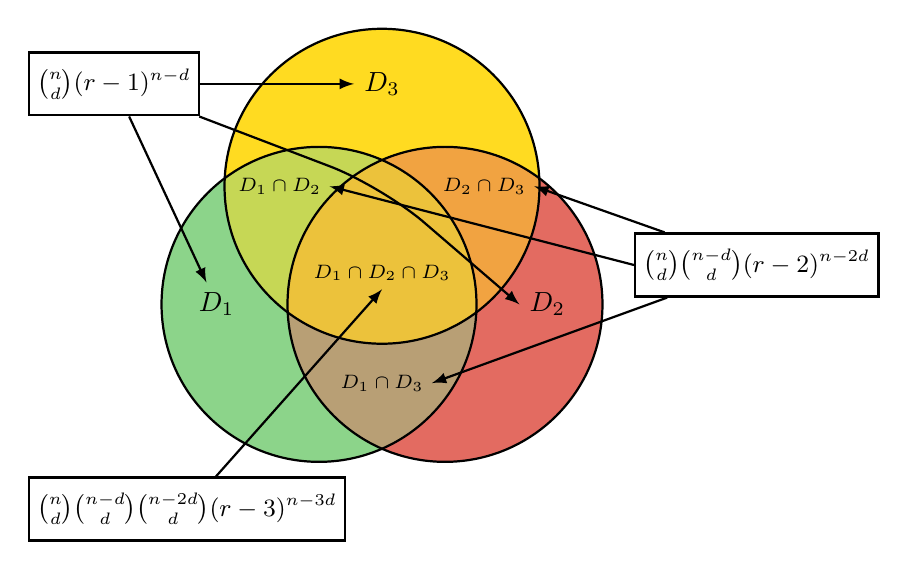
\begin{tikzpicture}[thick,
		set/.style = {circle,
			minimum size = 4cm,
			fill=blue}]
		
		\tikzstyle{formula}=[shape=rectangle,draw=black,fill=white,minimum width=1cm,minimum height=.8cm]
		
		% Set D1
		\node[set, fill=color1] (D1) at (0,0) {}; 
		
		% Set D2
		\node[set, fill=color2] (D2) at (1.6,0) {};
		
		% Set D3
		\node[set, fill=color3] (D3) at (0.8,1.5) {};
		
		% Intersection
		%% D1 D2
		\begin{scope}
			\clip (0,0) circle(2cm);
			\clip (1.6,0) circle(2cm);
			\fill[color1!50!color2](0,0) circle(2cm);
		\end{scope}
		
		%% D1 D3
		\begin{scope}
			\clip (0,0) circle(2cm);
			\clip (0.8,1.5) circle(2cm);
			\fill[color1!50!color3](0,0) circle(2cm);
		\end{scope}
		
		%% D2 D3
		\begin{scope}
			\clip (1.6,0) circle(2cm);
			\clip (0.8,1.5) circle(2cm);
			\fill[color2!50!color3](1.6,0) circle(2cm);
		\end{scope}
		
		%% D1 D2 D3 
		\begin{scope}
			\clip (0,0) circle(2cm);
			\clip (1.6,0) circle(2cm);
			\clip (0.8,1.5) circle(2cm);
			\fill[color1!33!color2!33!color3](0,0) circle(2cm);
		\end{scope}
		
		% Circles outline
		\draw (0,0) circle(2cm); 
		\draw (1.6,0) circle(2cm);
		\draw (0.8,1.5) circle(2cm);
		
		% Set label
		\node (D3) at (0.8,2.8) {$D_3$};
		\node (D2) at (2.9,0) {$D_2$};
		\node (D1) at (-1.3,0) {$D_1$};
		\scriptsize
		\node (D1D3) at (0.8,-1) {$D_1 \cap D_3$ };
		\node (D1D2) at (-0.5,1.5) {$D_1 \cap D_2$ };
		\node (D2D3) at (2.1,1.5) {$D_2 \cap D_3$ };
		\node (D1D2D3) at (0.8,0.4) {$D_1\cap D_2 \cap D_3$};
		
		%% formula 
		\small
		\node[anchor=west,formula] (F1) at (-3.7,2.8){$\binom{n}{d} (r-1)^{n-d}$};
		\node[anchor=west,formula] (F2) at (4,0.5) {$\binom{n}{d}\binom{n-d}{d}(r-2)^{n-2d}$};
		\node[anchor=west,formula] (F3) at (-3.7,-2.6) {$\binom{n}{d}\binom{n-d}{d}\binom{n-2d}{d} (r-3)^{n-3d}$};
		
		%% arrow linking the combinatorial formula to region.
		\draw[-latex] (F1)--(D1);
		\draw[-latex] {[rounded corners=20pt] (F1)--(0.8,1.5)--(D2.west)};
		\draw[-latex] (F1)--(D3);
		
		\draw[-latex](F2.west)--(D1D2.east);
		\draw[-latex](F2)--(D1D3.east);
		\draw[-latex](F2)--(D2D3.east);
		
		\draw[-latex] (F3) -- (D1D2D3.south);
	\end{tikzpicture}
	\caption{Ven diagram of the union of $3$ sets of $d-$colorful communities.}
	\label{fig:venn diagram union 3 sets}
\end{figure}

Figure~\ref{fig:venn diagram union 3 sets} shows the combinatorial formulas for all intersection cases of $3$ sets (see the Appendix for a detailed explanation of each formula). For $3$ sets the formula is thus:
\begin{equation*}
	3 \binom{n}{d} (r-1)^{n-d}-3 \binom{n}{d} \binom{n-d}{d} (r-2)^{n-2 d}+\binom{n}{d}
	\binom{n-d}{d} \binom{n-2 d}{d} (r-3)^{n-3 d},
\end{equation*}
which can be simplified by setting $r=3$ into:
$$\binom{n}{d} \left(\left(0^{n-3 d} \binom{n-2 d}{d}-3\right) \binom{n-d}{d}+3\ 2^{n-d}\right),$$
considering that $0^0=1$.

 Theorem~\ref{th:kappa} provides the general enumeration formula deduced from the Poincar\'e sieve once each intersection is combinatorically defined.

\begin{theorem}
The count of $d-$colorful communities of size $n$ with $r$ colors is given by $\kappa$ function: 
$$\kappa(r,n,d)=\sum _{k=1}^{\min \left(r,\left\lfloor \frac{n}{d}\right\rfloor \right)} \frac{(-1)^{k-1} \binom{r}{k} n! (r-k)^{n-k d}}{(n-k d)! (d!)^k}$$
\label{th:kappa} 
The proof is in the Appendix \qed
\end{theorem}


\subsection{Enumeration of the $d-$dominant colorful communities}
\label{sec:enumeration gamma}
\begin{figure}[p]
	\centering
	\begin{tikzpicture}
		\tikzstyle{formula}=[shape=rectangle,draw=black,fill=white,minimum width=1cm,minimum height=.8cm]
		\begin{scope}
			\node[inner sep=0] (sigdecomposition) at (0,0) {\includegraphics[width=0.9\textwidth]{image/comfromsig.png}};
		\end{scope}
		\node [anchor=south] (chrofun1) at (0,1.8) {\footnotesize \it Chromatic functions};
		\node [anchor=south,formula] (f1) at (0,0.8){$\frac{r!}{ \prod_{s \in \mathbf{Img}\circ \counts(\sigma)} s!}$};
		\node [anchor=south] (signature) at (0,-0.9) {\footnotesize \it Chromatic signatures};
		\node [anchor=south] (communities) at (0,5.7) {\footnotesize \it Communities};
		\node [anchor=south,formula] at (3,5.5)
		{$\frac{n !}{\prod_{k=1}^r \chi(k)!}$};
	\end{tikzpicture}
	
	\bigskip
	\begin{minipage}{0.9\textwidth}
		\small
		\textsc{parameters:} $r=3, n=5, d=$3. Two dominant signatures are deducted $(1,1,3)$ and $(0,2,3)$ which respectively correspond to $3$ and $6$ chromatic function groups. $20$ communities are associated with each chromatic function of the first group and $10$ for the second. A total of $120$ communities are $3-$dominant. The framed formulas correspond respectively to the number of chromatic functions of a signature (under ``Chromatic functions'') and to the number of communities dominant for a chromatic function (near ``Communities''). 
	\end{minipage}
	\caption{Enumeration of $3-$dominant communities of size $5$ with $3$ colors.}
	\label{fig:3-dominant communities}
\end{figure}
The domination implies to include the  dominance constraint in comparison to the $d-$colorful communities enumeration, leading to specify the different equivalence classes of communities complying with the dominations conditions~\ref{def:d dominant community}. Each class addresses the number of nodes for each color while fulfilling the dominance condition. 
Since the conditions of domination are only based on the number of vertices of the same color regardless the color, if two chromatic functions of two communities $p,q$ are equal up to a permutation on colors $\pi: C\to C$, 
$\chi_{c_p} = \pi \circ \chi_{c_q}$ then these communities share the same domination property. Thus they belong to the same equivalence class related to the color distribution.

 We introduce the notion of \emph{chromatic signature} $\sigma$ to capture this equivalence on chromatic functions. A signature of a chromatic function is a vector of color count corresponding to its ordered image (Definition~\ref{def: signature})
\begin{equation}
\sigma_p = \mathbf{Sort} \circ \mathbf{Img} \; \chi_{c_p}
\label{def: signature}
\end{equation} 
Several chromatic functions may have the same signature. For example the two chromatic functions: $\{1 \mapsto 0, 2 \mapsto 3, 3 \mapsto 2\}$ and $\{1 \mapsto 3, 2 \mapsto 0, 3 \mapsto 2\}$ have the same chromatic signature which is: $(0,2,3)$. 
The signatures are at he heart of the combinatorial formula enumerating the $d-$dominant coloring profiles by abstracting the chromatic functions. We can deduce that a signature of a $d-$dominant color profile complies with the following conditions: 
\begin{equation}
\left\{\begin{aligned}
&\sigma(r)=d \; \land \\
&\sum_{i=1}^r \sigma(i) = n \; \land \\
&\forall 1\leq i \leq r: \sigma(i) \leq d \;\land \\
&\forall 1 \leq i,j \leq r: i \leq j \implies \sigma(i) \leq \sigma(j). 
\end{aligned}\right.
\label{eq:domination conditions for signature}
\end{equation}
A chromatic signature properly defines an equivalence class on communities with regard to the domination property. Indeed, two communities with an equal chromatic signature share the same domination property (\ie $\sigma_p = \sigma_q \iff p \sim q$). Thus, each equivalence class specializing the property of domination according to the count of each color leads to a specific signature (Figure~\ref{fig:3-dominant communities}).
Let $\mathcal S_{r,n,d}$ be the set of all possible dominant signatures ($DSS$) with respect to parameters $r,n,d$, this set is explicitly generated by collecting all the signatures following Definition~\ref{eq:domination conditions for signature}. It represents the core of the combinatorial formula enumerating the $d-$dominant colorful communities. The algorithm computing this set is given in the Appendix.

Figure~\ref{fig:3-dominant communities} shows the distribution of the dominant colored communities into two equivalence classes distinguished by their color count. The communities are first grouped according to the chromatic function equality and next according to their signature equality by gathering the chromatic functions with the same signature. 
Counting all the $d-$dominant colorful communities intuitively follows this hierarchical division. From signatures, we first count the chromatic functions corresponding to them and then for each chromatic function we count the possible coloring profiles leading to this chromatic function. The final count of the dominant colorful communities is the product of these two steps. Theorem~\ref{th:gamma} defines the count of the $d-$dominant communities.

\begin{theorem}
The count of all possible $d-$dominant communities of size $n$ with $r$ colors is given by $\gamma$ function: 
$$\gamma(r,n,d)= n! r! \sum_{\sigma \in \mathcal S_{r,n,d}} \frac{1}{\prod_{s \in \mathbf{Img}\circ \counts(\sigma)} s! \; \prod_{i=1}^r\sigma(i)!}. $$
\label{th:gamma} 

The proof is in the Appendix. \qed
\end{theorem}


\subsection{Chromarity definition}
\label{sec:chromarity definition} 
From the enumeration of the (dominant) colorful communities, we can formally define the chromarity which somehow defines the random-free color density expectation. The \emph{core chromarity} ($\doot K$) applies the measure to a single community and provides a density weighted by the probability of the absence of chance. The higher the chromarity, the less likely it is to happen by chance. We first focus on the probability of getting a coloring profile by chance. This corresponds to the ratio of the favorable cases to the possible cases where the favorable cases is given by $\kappa$ or $\gamma$ while the number of all possible colorful communities is $r^n$. Therefore, for a community $p$ such that $n=|p|$ with a coloring profile $c_p$ distributing $r$ colors into vertices of $p$, and considering the largest number of vertices of the same color $d= \max \chi_{c_p}$. These probabilities are respectively: 
\begin{equation*}
	p_\kappa = \frac{\kappa(r,n,d)}{r^n} ,\; p_\gamma= \frac{\gamma(r,n,d)}{r^n}
\end{equation*}
The probability of getting a random-free coloring profile is thus $1-p_\kappa$ or $1-p_\gamma$. Therefore the core chromarities are defined as follows:
\begin{equation}
\begin{aligned}
\doot K_\kappa(r,n,d) &= \frac{d}{n} \left(1- \frac{\kappa(r,n,d)}{r^n} \right)\\
\doot K_\gamma(r,n,d) &=\frac{d}{n} \left(1- \frac{\gamma(r,n,d)}{r^n} \right)\\
\text{with} & \; r=|C|,\; n=|p|,\; d= \max \chi_{c_p} 
\end{aligned}
\label{def:core chromarity}
\end{equation}
We have $0\leq \doot K_{k_f}(r,n,d) \leq 1$. 

\medskip
For a community reduced to a single vertex (\ie $n=d=1$) with the maximal density of $1$ we can verify that $\doot K_\kappa(r,1,1)=\doot K_\gamma(r,1,1)=0$.
Similarly, for a single color coloring ($r=1$), the core chromarities are also null: $\doot K_\kappa(1,n,n)=\doot K_\gamma(1,n,n)=0$, (Proposition~\ref{prop:Kk=Kg=0}). These two results are consistent with the facts that in a singleton community or when a single color is used all the vertices of a community are necessary colored by a single color which can thus be obviously obtained by chance.

\begin{proposition} We have the following properties for $\doot K_\kappa$ and $\doot K_\gamma$:
\begin{itemize}
\item$\doot K_\kappa(r,1,1)=\doot K_\gamma(r,1,1)=0$.
\item $K_\kappa(1,n,n)=\doot K_\gamma(1,n,n)=0$.
\end{itemize}
The proof is in the Appendix. \qed
\label{prop:Kk=Kg=0}
\end{proposition}

When $p=\emptyset$ or $p$ is only composed of transparent vertices, either $|p|=0$ or $\max \chi_{c_p}$ is undefined, the density $\frac{\max \chi_p}{|p|}$ cannot be computed then preventing to return a proper result for $\doot K$. For these borderline cases, we do consider by convention that $\doot K(r,0,d)= \doot K(r,n,-\infty)=0$ to maintain the consistency of the measure.

The chromarity will be the mean of the core chromarity on a community structure $P$:
\begin{equation}
\begin{aligned}
K_\kappa(P,c) &= \frac{\sum_{p \in P} \doot K_\kappa(|C|,|p|,\max \chi_{c_p}) }{|P|}\\
K_\gamma(P,c) &= \frac{\sum_{p \in P} \doot K_\gamma(|C|,|p|,\max \chi_{c_p}) }{|P|}\\
\end{aligned}
\label{def:chromarity}
\end{equation}
We have $0\leq K_{\kappa}(P,c) \leq 1$ and $0\leq K_{\gamma}(P,c) \leq 1$ . 

\section{Chromatic community structure detection}
\label{sec:chrocode}
\begin{figure}[p]
	\begin{tikzpicture}
		%% FIGURES
		\begin{scope}
			\node[inner sep=10,anchor=north] (initialnet) at (1,0) {\includegraphics[width=0.25\textwidth]{image/GC2.png}};
		\end{scope}
		\begin{scope}
			.2 \node[inner sep=10,anchor=north] (step1) at (4.4,0) {\includegraphics[width=0.25\textwidth]{image/stepChroCoDe1.png}};
			\node[inner sep=10,anchor=north] (step2) at (8.,0) {\includegraphics[width=0.25\textwidth]{image/stepChroCoDe2.png}};
			\node[inner sep=10,anchor=north] (step3) at (8.,-5) {\includegraphics[width=0.25\textwidth]{image/stepChroCoDe3.png}};
			\node[inner sep=10, anchor=north] (step4) at (4.4,-5) {\includegraphics[width=0.25\textwidth]{image/stepChroCoDe4.png}};
		\end{scope}
		%% CHROMARITIES
		\begin{scope}
			\node[inner sep=2,anchor=south] (K1) at (4.4,-4.75) {$K_\gamma=0.57$};
			\node[inner sep=2,anchor=south] (K2) at (8.,-4.75) {$K_\gamma=0.74$};
			\node[inner sep=2,anchor=north] (K3) at (8.,-4.75) {$K_\gamma=0.91$};
			\node[inner sep=2,anchor=north] (K4) at (4.4,-4.75) {$K_\gamma=0.92$};
		\end{scope}
		
		\begin{scope}
			\node[inner sep=10,anchor=north] (finalnet) at (1,-4.5){\includegraphics[width=0.25\textwidth]{image/finalnet.png}};
		\end{scope}
		%% FLECHES AUTOUR
		\tikzset{
			arst/.style={
				draw, line width=15pt, black!20!white, {-Stealth[inset=0pt, angle=60:25pt]}, bend left=60,line cap=round, postaction=decorate, decoration={text along path, text color=black, text align=center, text={|\scriptsize|#1}}}}
		
		\begin{scope}
			\path [arst={Community Quotient Graph}] (initialnet.north) to (step1.north);
			\path [arst= { {$\lbrace$}III{$\rbrace$} {$\cup$} {$\lbrace$}IV{$\rbrace$} {$\cup$} {$\lbrace$}VII{$\rbrace$}} ] (5.5,0.2) to (8.4,0.);
			\path [arst= { {$\lbrace$}V{$\rbrace$} {$\cup$} {$\lbrace$}III, IV, VII{$\rbrace$}} ] (step2.east) to (step3.east);
			\path[arst={{$\lbrace$}II{$\rbrace$} {$\cup$} {$\lbrace$}V, III, IV, VIII{$\rbrace$}} ] (step3.south) to (step4.south);
			\path[arst={Chromatic Community Structure} ] (4.,-9) to (0,-8.);
		\end{scope}
	\end{tikzpicture}
	\begin{minipage}{0.9\textwidth}
		\footnotesize The labels of the cluster of nodes that are vertices of the quotient graph are in Roman while the nodes of the original graph are labeled in Arabic.
		
		\noindent
		\textsc{Parameters}: $n=25, \delta=2, r=4$.
	\end{minipage}
	\caption{\chrocode algorithm steps.}
	\label{fig:ChroCoDe steps}
\end{figure}
The chromatic community detection algorithm (\chrocode) finds a partition of a colored graph maximizing the chromarity $K$. The algorithm is divided in two phases: first a partition grouping connected nodes of the same color is built, forming as partition of monochrome communities, and next these communities are iteratively merged to increase the chromarity until no merges can improve the solution. 
The input parameters of the algorithm are the colored graph $G,c$, a neighborhood distance $\delta$, and a chromarity $K_\kappa$ or $K_\gamma$. The algorithm was originally inspired by the Louvain algorithm~\cite{blondel2008} although the specificity of the chromatic community structure framework leads to a significantly different program. \chrocode is freely distributed in two open-source implementations: in Python~\cite{chrocodePython} and in Mathematica-Wolfram~\cite{chrocodeMathematica}.
The algorithm is completely detailed in the Appendix. In more detail, the tasks carried out during these two stages are:
\paragraph{1) Connected monochrome community structure.} 
From a colored graph $\tuple{V,E,c}$, a community is designed from a vertex seed by first integrating neighboring vertices of the same color, then extending it by integrating their respective neighborhood having the same color and so on. Once no supplementary vertices can be added, the current community is closed and stored. Another  vertex is then chosen as seed until no vertices are available. The resulting community structure $P$ is composed of monochrome communities. 

\paragraph{2) Fusion of monochrome communities.}
From the monochrome communities $P$ previously obtained, we define a quotient graph $Q$ where each community becomes a node of this graph ($Q=\tuple{P,E_P}$). There exists a link between two community-nodes if there already exists a link between some nodes composing the respective communities ($E_P=\{ (p_i, p_j) \mid \exists (v_i, v_j) \in E: v_i \in p_i \land v_j \in p_j \}$).

Next the communities are merged to increase the chromarity. Iteratively, the community $p$ with the smallest core chromarity score is selected from $P$, and its neighborhood $N$ of distance $\delta$ is computed ($p \in \argmin_{p \in P} \doot K(|C|,|p|,\max \chi_{c_p})$). The algorithm evaluates whether merging $p$ to a neighbor node will improve the chromarity. $p$ is finally merged with  neighbor $q$ that maximally increase the current chromarity. The node-communities located in the shortest path from $p$ to $q$ are also merged in order to fulfill the connectedness rule within the new resulting community. Once the assembly of nodes is achieved they will now form a new community-node corresponding to their union. 

The quotient graph is then updated by replacing the merged nodes by this new node-community and by updating the quotient graph. The process ends when no merges improve the current chromarity.  

\medskip
Let $\tuple{G,E,c}$ be a colored graph, the complexity of the first phase is in $\mathcal{O}(|E|)$ since all nodes are visited from neighborhood to neighborhood to merge them into monochrome communities. Now considering the worst case for monochrome community reduced to a set of node singletons because the colors of all nodes are different, and assuming that at each step the new community merges only two communities, we deduce that the complexity is in $\mathcal{O}(|V|^2(|E|+|V|\log(|V|)))$.

Figure~\ref{fig:ChroCoDe steps} shows the evolution steps of the algorithm. First the monochrome community quotient graph is defined. Let us remark that two connected node-communities have necessary a different color. Next the algorithm starts by merging the reduced single-node communities into larger communities because their chromarity is $0$ constituting the lowest possible value. After, the communities are grouped together for forming larger communities increasing the chromarity since it evolves from $0.57$ to $0.92$. 

Figure~\ref{fig:big example} shows the computation steps on a larger example of $50$ nodes where the curve describes the chromarity progression by indicating the community assemblies at each step and the community improvement ($y-$axis). The grid graph was chosen because it provides a clean presentation of the final communities on the graph but the algorithm can be applied to any graph.
\begin{figure}[ht]
	\centering
	\includegraphics[height=0.4\textheight]{image/bigexample.png}
	\begin{minipage}{0.9\textwidth}
		\footnotesize Upper left: initial quotient graph of monochrome communities; lower right: the colored graph where each final community contains the vertices with the same color border; below each step point of the curve: the communities to be merged, a column of roman numbers indicates a previously merged community.
		
		\noindent
		\textsc{Parameters}: $n=50, \delta=2,r=4, K_\gamma$.
	\end{minipage}
	\caption{Chromatic community structure computation.}
	\label{fig:big example}
\end{figure}

\section{CHROCODE evaluation}
\label{sec:benchmark}

 \chrocode will be analyzed with regard to three network topologies: small world, scale free, and Erd\"os Reny. the exploitation of these different network topologies allows us the assessment of their respective influence on the performance of the algorithm.
%\begin{figure}[htb]
%	\begin{tabu}{ X[c] X[c] X[c]}
%		\includegraphics[width=0.3\textwidth]{image/gsw.png} &\includegraphics[width=0.3\textwidth]{image/gsf.png} & \includegraphics[width=0.3\textwidth]{image/ger.png}\\
%		\textsc{small world} & \textsc{scale free} & \textsc{Erd\"os Reny}
%		%% \\ \footnotesize Rewiring probability$=0.3$. & \footnotesize $+$ vertex with $3$ edges. & \footnotesize $15\%$ of edges.
%	\end{tabu}
%	\caption{Network Topology Examples}
%	\label{fig:topology}
%\end{figure}

\subsection{Chromarity analysis}
 The choice of the chromarity $K_\kappa$ or $K_\gamma$ seemingly alters the community structure obtained by \chrocode algorithm. How significant can this difference be? 
This issue is crucial because the computational time between $K_\kappa$ or $K_\gamma$ could drastically differ. 
The complexity of $\doot K_\kappa$ is in $\mathcal{O}(r n)$ while the complexity of $\doot K_\gamma$ depends on the cardinality of the $DSS$ $\mathcal S$, in $\mathcal{O}(|\mathcal S| r n)$. Figure~\ref{fig:dominant set variation} shows the evolution of the cardinality of the $DSS$ by choosing optimally the parameters $r,n,d$ to maximize its growth. Notice that the optimal $r$ is $r=n-d+1$. 

The size of the $DSS$  grows exponentially when $n$ increases by selecting the optimal parameters $r,d$ (see Figure~\ref{fig:dominant set variation}.1 ). However it is also worth noting that this growth is limited if $r$ remains small ($\lesssim 10$) (Figure~\ref{fig:dominant set variation}.3) which is often the case in practice. 
\begin{figure}[htb]
	\footnotesize
	\centering
	\begin{tabu}{X[c] X[c]}
		\multicolumn{2}{c}{1) $n-$evolution with optimal $r$ and $d$.} \\
		\multicolumn{2}{c}{\includegraphics[width=0.5\textwidth]{image/ngrowth}} \\
		2) $d-$evolution & 3) $r-$evolution \\
		\includegraphics[width=0.45\textwidth]{image/optimald.png}& 
		\includegraphics[width=0.45\textwidth]{image/optimalr.png}\\
		$n=50, r=n-d+1$. & $n=50, d=11$. 
	\end{tabu} 
	\caption{Evolution of the cardinality of the $DSS$ $\mathcal S$.}
	\label{fig:dominant set variation}
\end{figure}

Hence when the computation of the $DSS$ is intractable due to its size, we do wonder know if we can validly use $K_\kappa$ instead of $K_\gamma$. 
To answer to this question we compare the chromarities of the community structure computed by \chrocode using respectively $K_\kappa$ and $K_\gamma$ as input ((Figure~\ref{fig:K difference}).
\begin{figure}[p]
	\begin{center}	
		\footnotesize
		1) Chromarity difference $\Delta_K$ based on \chrocode computation.
		
		\includegraphics[width=0.7\textwidth]{image/diffK.png}
		
		2) Core Chromarity difference $\doot \Delta_K$.
		
		\begin{tabu}{X[c,p] X[c,p]}
			\includegraphics[width=0.45\textwidth]{image/plotdiffK.png} & \includegraphics[width=0.45\textwidth]{image//plotNdiffK.png}\\
			Evolution of $\doot \Delta_K$ w.r.t. $n,d$ & Mean difference of non-null $\doot \Delta_K$.
		\end{tabu}
		
		\medskip
		
		\begin{minipage}{0.8\textwidth}
			\footnotesize 
			1) The analysis is achieved on $49$ different cases ($r=4, \delta=2$).
			
			2) $1275$ differences are computed since $d$ never exceeds $n$. For the mean difference computation (at right), the zero values are removed unless only this value exists. The error bar represents the standard error.
		\end{minipage}
	\end{center}
	
	\caption{Chromarity difference}
	\label{fig:K difference}
\end{figure}

For each topology we generate $10$ networks by increasing their size from $10$ to $100$ by $10$. Therefore for each topology $100$ networks are produced ($300$ networks in total). For the benchmark, we use $4$ colors ($r=4$) and a neighborhood of distance $2$ ($\delta=2$).
Based on these networks, we isolate the cases where the resulting community structure computed by \chrocode differs using $K_\kappa$ or $K_\gamma$ leading to two distinct community structures depending on the used chromarity: $P_\kappa = \Call{chrocode}{G,c,\delta, K_\kappa}$ and $P_\gamma=\Call{chrocode}{G,c,\delta, K_\gamma}$ with $P_\kappa \neq P_\gamma$. 

The percent of networks where the community structures differ closely depends on the topology. The small world topology induces more differences than the other topologies. We determine the \emph{chromarity distance} which is the chromarity difference between the respective community structures: $\delta_K=| K(P_\gamma,c)-K(P_\kappa,c)|$ for both chromarities $K_\kappa$ and $K_\gamma$. Even a community structure is deduced from a specific chromarity we can compute the other chromarity on this structure. Figure~\ref{fig:K difference}.1 describes the observed distances. The chromarity distance never exceeds $0.08$ with the tested networks whatever the topologies and the chosen chromarity. Therefore, the difference between the chomarities depends on the network topologies but seemingly remains moderate on the tested cases. 

Moreover, we have also directly evaluated the core chromarity distance $\doot \Delta_K$ by making $n,d$ varying with the optimal parameter for $r=n-d+1$ (Figure~\ref{fig:K difference}.2). This evaluation is focused on the difference between the chromarities and not the impact on \chrocode computation, providing a complementary approach to the previous one. This evaluation shows that the difference is significant when $d$ is small and bounded by $0.23$. The decrease of the mean of $\doot \Delta_K$ is exponential and becomes negligible when $n > 10$ since $\overline{\doot \Delta_K} \leq 0.05$. Moreover when $d>5$ we have $\doot \Delta_K \leq 10^{-5}$ whatever the value of $n$. 

In conclusion, from these two evaluations, the quality of the community structures appears almost equivalent whatever the chromarity used. Hence, the chromarities can be somehow considered practically similar although their definition differ. 

\subsection{Network size sensitivity} 
The efficiency of the algorithm is sensitive to the network topology and its size. 
Figure~\ref{fig:Network size sensitivity} clearly shows that the chromarity improves when the size increases and the topology also accounts in the chromarity score. The best chromarity is obtained on Erd\"os Reny topology. The curves of the chromarities are similar because a real difference between them occur only when \chrocode provides different community structures according to the used chromarity. We have previously shown that that only few cases induced a difference and the chromarity distance remains low 
(Figure~\ref{fig:K difference}.2). 

\begin{figure}[htb]
	\centering
	\footnotesize
	\begin{tabu}{X[c,p] X[c,p]}
		\includegraphics[width=0.4\textwidth]{image/klk.png} & \includegraphics[width=0.4\textwidth]{image/klg.png}\\
		$K_\kappa$ & $K_\gamma$\\
		\multicolumn{2}{c}{\includegraphics[width=0.45\textwidth]{image/klegend.png}}
	\end{tabu}
	\begin{minipage}{0.9\textwidth}
	\footnotesize 		
	The curves correspond to the mean of the chromarity on $10$ trials and the error-bars describe the standard error. ($r=4,\delta=2$). 
\end{minipage}
\caption{ Evolution of the chromarity w.r.t. the vertex size.}
\label{fig:Network size sensitivity}
\end{figure}

\subsection{Neighborhood distance} The variation of the distance of the neighborhood ($\delta$) also affects the final result. Figure~\ref{fig:Neighborhood distance} shows the consequence of the variation of the neighborhood distance from $1$ to $10$ on the chromarities with $10$ networks of size $100$ for each value of $\delta$ on different topologies. for each trial \chrocode was computed twice using both chromarities and the community structure with the smallest chromaty is kept when the result differs.
 We can observe that the optimal distance $\delta$ differs on the topologies. The optimal $\delta$ is $3$ for Small world networks while it is $1$ for Scale Free, and the variation of $\delta$ does not significantly affect the result for Erd\"os Reny topology. It is also worth noticing that the variation is always stabilized after $\delta=5$ for all network trials. 

Therefore, a possible improvement of the algorithm regardless the network topology is to perform $5$ tests by varying $\delta$ from $1$ to $5$ and to keep the structure with the highest chromarity among these tests.
\begin{figure}[htb]
	\centering
	\footnotesize
	\begin{tabu}{X[c,p] X[c,p]}
		\includegraphics[width=0.4\textwidth]{image/deltak.png} & \includegraphics[width=0.4\textwidth]{image/deltag.png}\\
		$K_\kappa$ & $K_\gamma$ \\
		\multicolumn{2}{c}{\includegraphics[width=0.45\textwidth]{image/klegend.png}}
	\end{tabu}
	
	\begin{minipage}{0.9\textwidth}
		\footnotesize 		
	The diagram reports the mean of the chromarity on $10$ trials of networks of size $100$ and the error-bars describe the standard error. A different network is generated for each trial.
		%% The percent of community structure difference between chromarities is respectively: Small world $18\%$, Scale Free $3\%$, Erd\"os Reny $1\%$. 
		( $r=4, |V|=100$).
	\end{minipage}
	
	\caption{Impact of $\delta$ on \chrocode result.}
	\label{fig:Neighborhood distance}
\end{figure}
\section{Conclusion}
\label{sec:conclusion}
We propose a new approach to detecting communities that relies on new criteria to identify them. Instead of a difference in connection density between its interior and its border, defining a community will maximize the density of nodes sharing the same property. By assimilating property to color, we will therefore seek to maximize the density of nodes of an identical color within each community.

This new paradigm provides an alternative approach to connectivity rule. It takes on its full meaning in challenges where the connection of nodes sharing the same property remains loose and therefore cannot be captured by an examination of the connection density as has been shown for disease modules. 

This clustering criterion appears natural and finds its application in problems where the community organization is essentially based on the aggregation of nodes sharing the same property without apparent correlation with the law of connectivity.

We characterize two chromarity measures assessing the quality of a community structure comparing the major color density with that which would have been calculated for a random network with identical characteristics. High degree of chromarity means that the community structure cannot have been the result of chance confirming its organizational relevance. We have proposed a \chrocode heuristic solving this problem in polynomial time. The tests analyzing the performance of this algorithm highlight the proximity of the two chromarities as well as a very good performance of the algorithm. 

A first perspective would be to improve the algorithm by refining the heuristic criteria for better aggregating communities.  Another perspective would be to study how the grouping of nodes according to the major color rule could also integrate connectivity between nodes of the same color. Indeed, sharing the same property, these nodes could develop a particular connectivity structure characterizing a connection pattern that can be specific to the shared property. Such a perspective would allow recognition of a property-dependent community through an hybrid model, combining the identical property recognition with connectivity rules for detecting communities.
 
\clearpage
\section*{Appendix}

\subsection*{Proofs}

\begin{proof}[Proof of Theorem~\ref{th:kappa}]
To combinatorially specify the cardinality of $|\bigcup_{k=1}^r D_k|$, we need to determine the cardinality of all the intersection sets $|\bigcap_{k=l}^m D_k|, 1 \leq m \leq r$. We illustrate the characterization of the formulas on $3$ sets before generalizing it to ease the explanation. The main issue is to formulate the cardinality of any intersection of set by a combinatorial formula. 

Basically $D_k=\{ p \mid \exists k \in c: \chi_{c_p}(k) = d \}$ is a set of communities with $d$ vertices of color $k$. The different possible selections of $d$ vertices among $n$ is given by $\binom{n}{d}$. The count of the rest of the profile once the color $k$ is assigned to vertices equals $(r-1)^{n-d}$, leading to the following combinatorial characterization of $|D_k|$:
\begin{equation*}
|D_k|= \binom{n}{d}(r-1)^{n-d}.
\label{eq: DK combinatorial formula}
\end{equation*}
Let us remark that this formula can be applied for all the colors and the number of possible used color is $\binom{r}{1}$ (which is $3$ for $r=3$). We deduce that $|D_1|+ |D_2| + |D_3|= \binom{r}{1} \binom{n}{d}(r-1)^{n-d} =3 \binom{n}{d} 2^{n-d}.$

By extension, for the intersection of two sets $D_k \cap D_j= \{ p \mid \chi_{c_p}(k) = d \land \chi_{c_p}(j) = d \}$ the cardinal is defined by first considering the selection of a subset of size $d$ for color $k$ and next the selection of a size $d$ vertices of color $j$ in the remaining $n-d$ vertices. The following combinatorial formula formalizes these two steps of vertices selection.
\begin{equation*}
|D_k \cap D_j|= \binom{n}{d} \binom{n-d}{d}(r-2)^{n-2d}.
\label{eq: DK inter Dj combinatorial formula}
\end{equation*}
Similarly, the number of possible color pairs is given by $\binom{r}{2}$ (which is $3$ for $r=3$).
Then, we conclude that: 
\begin{equation*} 
D_1 \cap D_2| + |D_1 \cap D_3| + |D_2 \cap D_3| = \binom{r}{2} \binom{n}{d} \binom{n-d}{d}(r-2)^{n-2d} = 3 \binom{n}{d} \binom{n-d}{d}.
\end{equation*}
The same reasoning can be applied for the cardinal of the intersection of the three sets $|D_1 \cap D_2 \cap D_3|$ and more generally for any intersection.
\begin{equation*}
|D_1 \cap D_2 \cap D_3|=\binom{r}{3}\binom{n}{d} \binom{n-2 d}{d} \binom{n-d}{d} (r-3)^{n-3 d}
\end{equation*}
The formula holds under considering that $0^0=1$ since $(r-3)^{n-3d}=0^{n-3d}$ which must not be null or undefined when $n=3d$ \eg for $r=3,n=6,d=2$ we have $|D_1 \cap D_2 \cap D_3|=90$.
The formula defining the cardinal of the union of the $3$ sets is finally: 

\begin{multline*}
|D_1 \cup D_2 \cup D_3|= \binom{r}{1}\binom{n}{d}(r-1)^{n-d} \\ - \binom{r}{2} \binom{n}{d} \binom{n-d}{d}(r-2)^{n-2d} \\ + 
\binom{r}{3} \binom{n}{d} \binom{n-d}{d}\binom{n-2d}{d}(r-3)^{n-3d}.
\end{multline*}

The generalization to any number of colors based on the Poincar\'e sieve finally leads to: 
\begin{equation*}
\left|\bigcup_{k=1}^r D_k \right|= \sum _{k=1}^r (-1)^{k-1} \binom{r}{k} \left(\prod _{i=0}^{k-1} \binom{n-i d}{d}\right) (r-k)^{n-k d}.
\end{equation*}
By simplification of the product and by considering that the product is null if $r d> n$ the number of $d-$ colorful communities of size $n$ with $r$ colors is finally given by $\kappa$ function.
\begin{equation*}
\kappa(r,n,d)=\sum _{k=1}^{\min \left(r,\left\lfloor \frac{n}{d}\right\rfloor \right)} \frac{(-1)^{k-1} \binom{r}{k} n! (r-k)^{n-k d}}{(n-k d)! (d!)^k} \qed
\end{equation*}

\end{proof}
\begin{proof}[Proof of Theorem~\ref{th:gamma}]
The enumeration of $d-$dominant communities is based on $DSS$ by applying the formula counting the number of permutations with repetition. Considering $m$ distributed on $n>m$ positions having each $k_i, 1 \leq i \leq m$ repetitions, the $n$ elements having each $k_i$ repetitions such that $\sum_{i=1}^m k_i = n$,  let us recall that the number of permutation with repetition is: 
\begin{equation*}
	\frac{n!}{\prod_{i=1}^m k_i!}
\end{equation*}

Indeed, first we count the number of color profiles of size $n$ for a specific chromatic function. 
Since the vertices of the same color cannot be distinguished in a community, the number of communities having the same chromatic function corresponds to the number of permutations where the vertices of the same color are repeated, that is:
\begin{equation*}
\frac{n !}{\prod_{k=1}^r \chi(k)!}
\end{equation*}
Notice that we can similarly define it using the signature $\sigma$ by $\frac{n !}{\prod_{k=1}^r \sigma(k)!}$. This formula using the signature $\sigma$ will be used in the sequel. 

\medskip 
Next we need to enumerate all the chromatic function related to a signature. Let us remark 
that the number of chromatic function with the same signature is also obtained by the application of a permutation with repetition. The repetition comes from the possible equality  of the number of vertices for distinct colors, thus decreasing the number of different chromatic functions. For example in Figure~\ref{fig:3-dominant communities}, the number of chromatic functions for $(1,1,3)$ is $3$ while it is $6$ for $(0,2 ,3)$ because there is a repetition of the number $1$ in the first and none in the second. Therefore, the formula counting chromatic functions taking into account the equal number of occurrences for different colors is:
\begin{equation*}
\frac{r!}{ \prod_{s \in \mathbf{Img}\circ \counts(\sigma)} s!}
\end{equation*} 

Finally, the number of communities associated to a signature is then the product of these two formulas, leading to: 
\begin{equation*}
\frac{n! r!}{\prod_{s \in \mathbf{Img}\circ \counts(\sigma)} s! \; \prod_{j=1}^r\sigma(j)!} 
\label{eq:count from signature}
\end{equation*}

This formula counts the number of communities having the same signature. The total number of communities is the sum of this count for all signatures. Let $\mathcal S_{r,n,d}$ be the $DSS$ according to parameters $r$ for the number of colors, $n$ for the community size and $d$ for the maximal number of vertices of the same colors, the formula counting the dominant communities is finally given by $\gamma$ function:

\begin{equation*}
\gamma(r,n,d)= n! r! \sum_{\sigma \in \mathcal S_{r,n,d}} \frac{1}{\prod_{s \in \mathbf{Img}\circ \counts(\sigma)} s! \; \prod_{i=1}^r\sigma(i)!}. \qed
\end{equation*}
\end{proof}


\begin{proof}[Proof of Proposition~\ref{prop:Kk=Kg=0}]
We prove that $\doot K_\kappa(r,1,1)=\doot K_\gamma(r,1,1)=0$. 

\medskip
\noindent
$\bullet$~By definition of $\doot K_\kappa$, we have:

\medskip
\begin{tabu} to \textwidth {X[0.1,$$] X[2,$$] X[1]}
\doot K_\kappa &= \frac{d}{n} \left(1- \frac{\kappa(r,n,d)}{ r^n} \right) \\
&= \frac{d}{n} \left(1- \frac{\sum _{k=1}^{\min \left(r,\left\lfloor \frac{n}{d}\right\rfloor \right)} \frac{(-1)^{k-1} \binom{r}{k} n! (r-k)^{n-k d}}{(n-k d)! (d!)^k}}{ r^n} \right) & set definition of $\kappa$;\\
&= 1- \frac{ \frac{(-1)^{0} \binom{r}{0} 0! (r-0)^{1 - 0 1}}{(0)! (1!)^0}}{ r} . & change $d,n$ by $1$;\\
&= \left(1- \frac{ r}{ r} \right) &By considering that $x^0=1, 0!=1, \binom{x}{0}=1, r>0$.\\
&=0 &\qed
\end{tabu}

\medskip
\noindent
$\bullet$~By definition of $\doot K_\gamma$, we have:

\begin{tabu} to \textwidth {X[0.1,$$] X[3,$$] X[1]}
\doot K_\gamma &= \frac{d}{n} \left(1- \frac{\gamma(r,n,d)}{ r^n} \right) \\
&= \frac{d}{n} \left(1- \frac{n! r! \sum_{\sigma \in \mathcal S_{r,n,d}} \frac{1}{\prod_{s \in \mathbf{Img}\circ \counts(\sigma)} s! \prod_{i=1}^r\sigma(i)!}}{ r^n} \right) & set definition of $\gamma$;\\
&= 1- \frac{1! r! \sum_{\sigma \in \mathcal S_{r,1,1}} \frac{1}{\prod_{s \in \mathbf{Img}\circ \counts(\sigma)} s! \; \prod_{i=1}^r\sigma(i)!}}{ r^1} & set $d=n,r=1$;
\end{tabu}

\hspace{4ex} As $\mathcal S_{r,1,1}=\{(\overbracket{0,\cdots,0}^{r-1},1) \}$, we deduce that: 

\hspace{4ex} $\prod_{s \in \mathbf{Img}\circ \counts(\sigma)} s! = (r-1)! 1!$ and $\prod_{i=1}^r\sigma(i)!= 1,$ 
thus leading to:

\medskip 
\begin{tabu} to \linewidth {X[0.1,$$] X[3,$$] X[1]}
\doot K_\gamma & = 1- \frac{1! r! \frac{1}{(r-1)!1! 1!}}{ r^1} & \\
& = 1- \frac{r!}{(r-1)!r} & by simplification\\
& = 1- \frac{r!}{r!} & by simplification\\
&= 0 & 
\end{tabu}
The proof that $\doot K_\kappa(1,n,n)=\doot K_\gamma(1,n,n)=0$ is similar and let to the reader. 
\end{proof}

\clearpage
\subsection*{CHROCODE Algorithm}
The main variables and used functions are:

{\footnotesize
\begin{tabu}{ |l X[l]}
$\Call{Vget}{V}$ &gets a vertex in $V$ (randomly). \\
$\Call{Path}{G}$ &set of pathes of graph $G$.\\
$\Call{ShortestPath}{ E,p,q}$ & finds a shortest path between $p,q$.\\
$P$ &Community structure. \\
$N$ & Neighborhood of distance $\delta$.\\
$up$ &Boolean variable determining whether $P$ must be updated.
\end{tabu}
}
%% \begin{algorithm}
\bigskip	
\noindent
The \chrocode function is:	
\begin{algorithmic}
\footnotesize
\Function{ChroCoDe}{$G=\tuple{V,E},c,\delta,K$}
\State $W \gets V$; 
\While{$W \neq \emptyset$} \Comment{Generate the monochrome communities.}
\State $v \gets \Call{Vget}{W}$; $W \gets W \setminus \{v\}$; 
\State $p_{\text{new}} =\{v\}$;$p = \emptyset$; 
\While {$p_{\text{new}} \neq \emptyset$} 
\State $w \gets \Call{Vget}{p_{\text{new}}}$; $p_{\text{new}} \gets p_{\text{new}} \setminus \{w\}$;
\State $p \gets p \cup \{w\}$; 
\State $N \gets \{ w' \mid (w,w') \in E \land c(w')=c(v) \land w' \notin p \}$; 
\State $p_{\text{new}} \gets p_{\text{new}} \cup N$;
\EndWhile
\State $W \gets W \setminus p$;
\State $P \gets P \cup \{p\}$;
\EndWhile \Comment $\tuple{P, E_P}$ is the quotient graph.
\State $ E_P \gets \{(p,p') \mid \exists v \in p, \exists v' \in p': (v,v') \in E, p,p' \in P\}$;
\State $W \gets P$;
\While{$W \neq \emptyset$} \Comment{Assemble the communities.}
\State $p \gets \argmin \; \{ \doot K(q,c) \mid q \in W\}; W \gets W \setminus \{p\}$; 
\State $N \gets \{q \mid q \in E_P \land 1 < \Call{ShortestPath}{E_P,p,q} \leq \delta \}$;
\State $k_{\max} \gets K(P,c)$; $up \gets False$;
\For{$q \in N$} \Comment{Find the merging of communities maximizing $K$ in $N$.}
\State $SP \gets \Call{ShortestPath}{ E_P,p,q}$;
\State $k \gets K( (P \setminus SP) \cup \left \{\bigcup_{p_i \in SP} p_i \right\},c)$; 
\If{$k_{\max} < k$}
\State $up \gets True$;
\State $k_{\max} \gets k$; $SP_{\max} \gets SP$;
\EndIf
\EndFor
\If{$up$}
\State $p= \bigcup_{p_i \in SP_{\max}} p_i$; \Comment{Merge the communities of the path.}
\State $ P \gets \left( P \setminus SP_{\max} \right) \cup \{p\}$; \Comment{Update P}
\State $ E_P \gets \{(p,p') \mid \exists v \in p, \exists v' \in p': (v,v') \in E, p,p' \in P\}$; \Comment{quotient graph rebuilt}
\State $W \gets P$;
\EndIf
\EndWhile
\State \Return $P$;
\EndFunction
\end{algorithmic}
%\caption{Chromatic Community Structure Detection Algorithm}
%\label{algo:ChroCoDe}
%\end{algorithm}

\clearpage
\subsection*{Algorithm computing the Dominant set of signatures ($DSS$)}
We define $.$ is the concatenation operator between two vectors, and a vector is written $(x_1,\cdots,x_m)$. 

\begin{algorithmic}
\algnewcommand\algorithmicto{\textbf{to}}
\algrenewtext{For}[3]%
{\algorithmicfor\ $#1 \gets #2$ \algorithmicto\ $#3$ \algorithmicdo}
\Function{SubSig}{$r,n,d,\sigma$}
\State{$\mathbf{var}: s$}
\If{$n=0$}
\State{$s \gets \{\overbrace{(0,\cdots,0)}^r . \sigma\}$}
\ElsIf{$d=0$}
\State{$s \gets \emptyset $}
\ElsIf{$r=1 \land n \leq d $} 
\State{ $s \gets \{(n) . \sigma\}$}
\ElsIf{$r=0 $}
\If{$n=0$}
\State{$s \gets \{\sigma\}$}
\Else
\State{$s \gets \emptyset$}
\EndIf
\Else
\State{$s \gets \emptyset$}
\For{d'}{\lceil \frac{n}{r} \rceil}{\min (d,r)}
\State{$s \gets s \cup \textsc{SubSig}(r-1, n -d', d', (d'). \sigma)$}
\EndFor
\EndIf

\Return{s}
\EndFunction

\bigskip
\Function{FindAllSigs}{$r,n,d$}
\State{$\mathbf{var}: S$}
\If{$r=0$}
   	\If{$n=0$}
   		\State{$S \gets \{\emptyset\}$} \Comment{a solution exists but empty}
  	\Else
  		\State{$S \gets \emptyset$} \Comment{No solutions}
  	\EndIf
\Else
	\State{$S \gets \textsc{SubSig}(r-1, n-d, d, \left(d\right))$}
\EndIf
\State \Return{$S$}
\EndFunction
\end{algorithmic}

\clearpage
\printbibliography
\end{document}